\section{圖片的壓縮}
  \subsection{研究目標}
  所謂圖片壓縮,就是以更小的容量儲存同一張圖片。本次實驗以臺大校徽作為研究對象,探討取樣數的多寡對壓縮後的圖片品質之影響。
  \\\\
  而因為每張圖片的總邊緣像素都不盡相同,本次報告以像素使用率作為研究指標:
  \[\text{像素使用率\,}r=\frac{\text{DFT\,中使用之像素}}{\text{總邊緣像素}}\eqno{(4.1)}\]
  
  \subsection{研究結果}
  當\,\(r=1\)\,時,程式的輸出圖像如圖\,6\,所示:
  \begin{figure}[h!]
  \centering
    \begin{minipage}{0.4\linewidth}
      \centering
      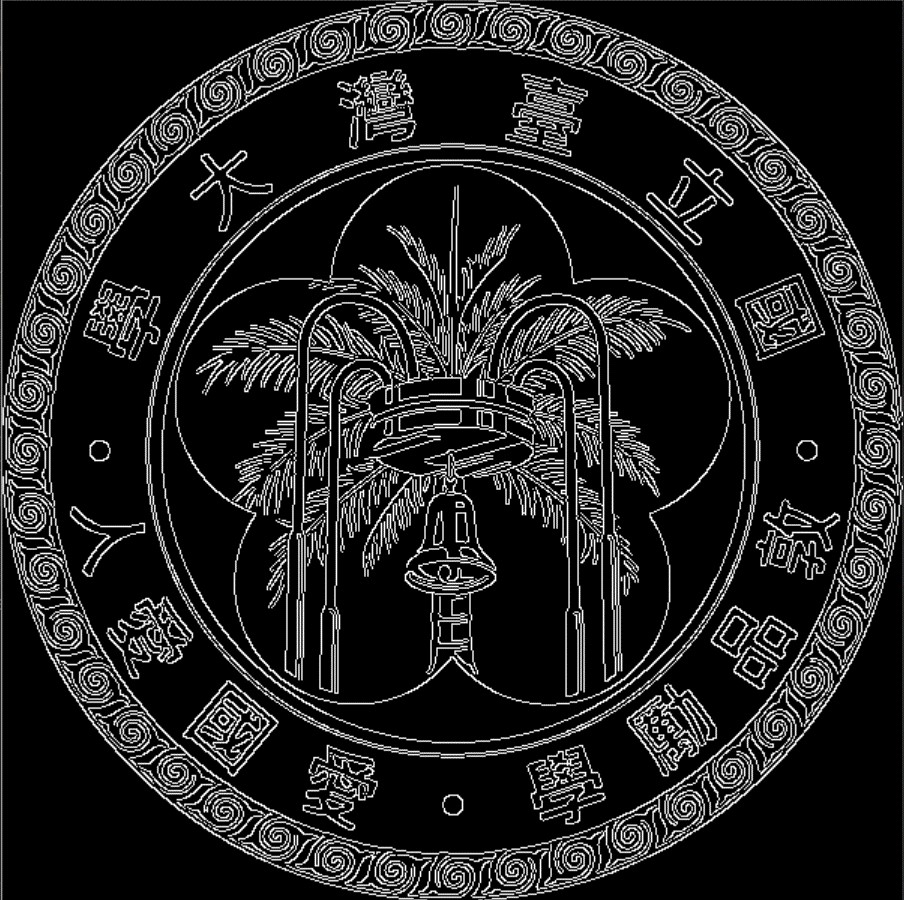
\includegraphics[width=150pt]{NTU edge.jpg}
      \caption*{\textbf{圖\,5}\(\quad\)Canny\,後的臺大校徽}
    \end{minipage}
    \quad
    \begin{minipage}{0.4\linewidth}
      \centering
      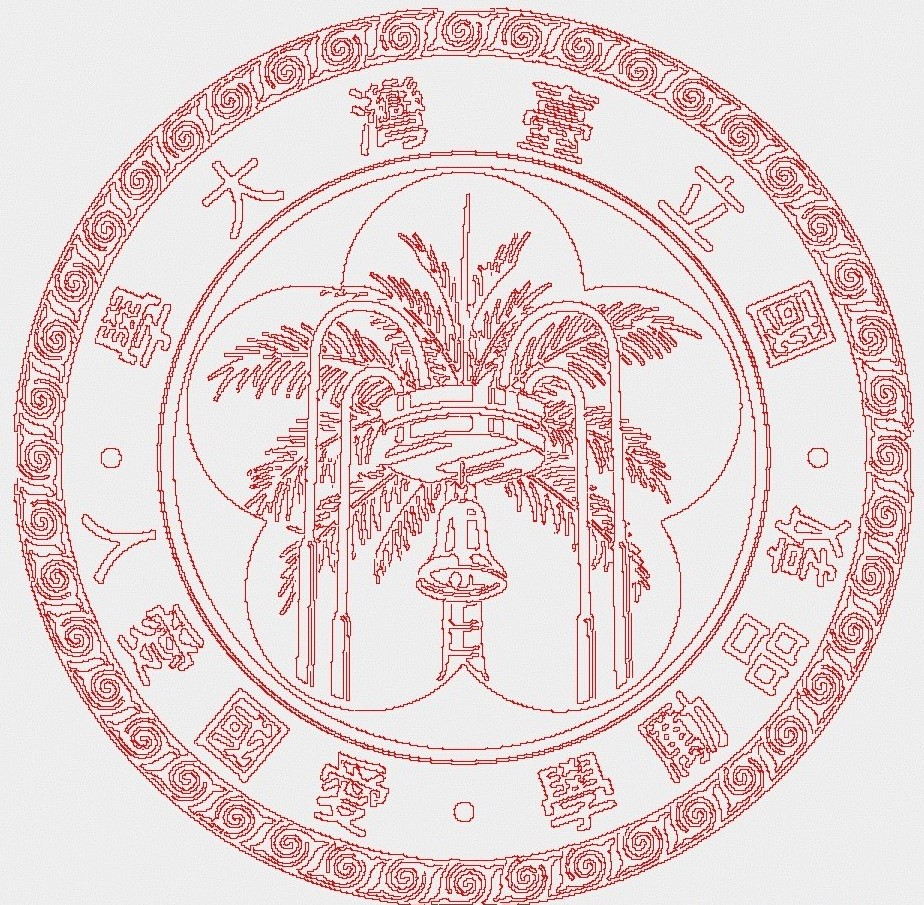
\includegraphics[width=150pt]{NTU r=1.jpg}
      \caption*{\textbf{圖\,6}\(\quad\)\(r=1\)\,時的輸出}
    \end{minipage}
  \end{figure}
  \noindent 可以看到此時的結果與圖\,(d)\,如出一轍,即\,DFT\,與\,IDFT\,成功了重現了原圖的所有資訊。
  \\\\
  接著我們逐次下降\,\(r\)\,值:\noindent
  \begin{figure}[h!]
  \centering
    \begin{minipage}{0.3\linewidth}
      \centering
      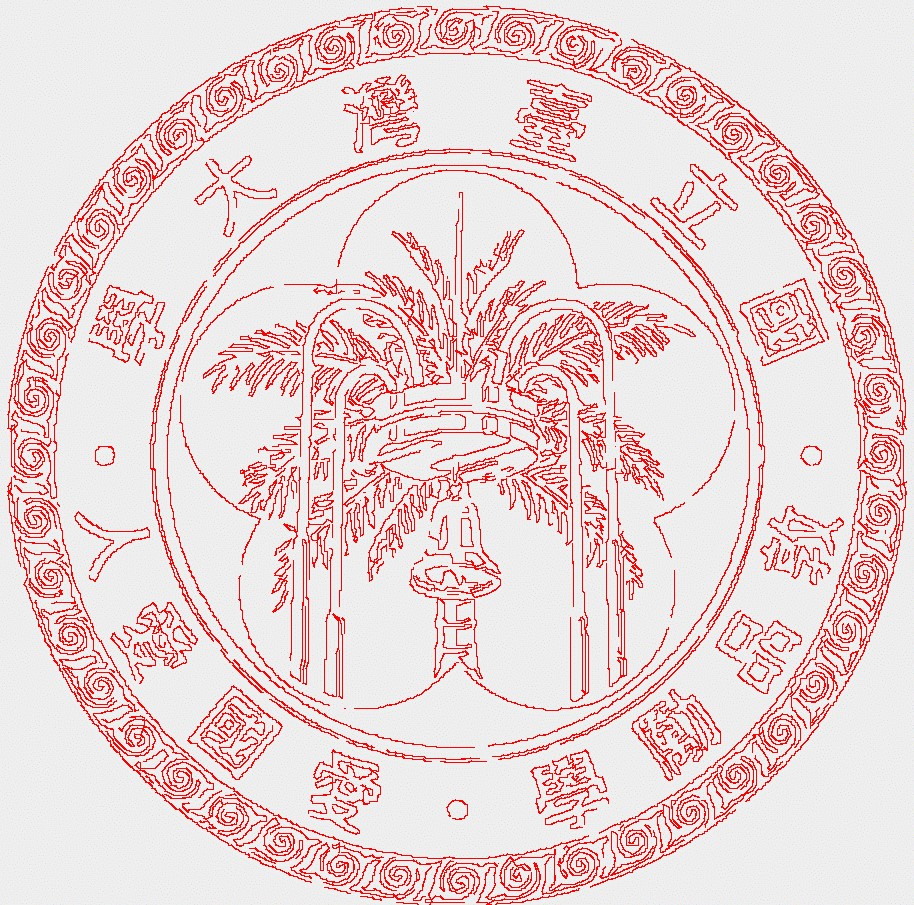
\includegraphics[width=120pt]{NTU r=0.7.jpg}
      \caption*{\textbf{圖\,7}\(\quad\)\(r=0.7\)\,時的輸出}
    \end{minipage}
    \quad
    \begin{minipage}{0.3\linewidth}
      \centering
      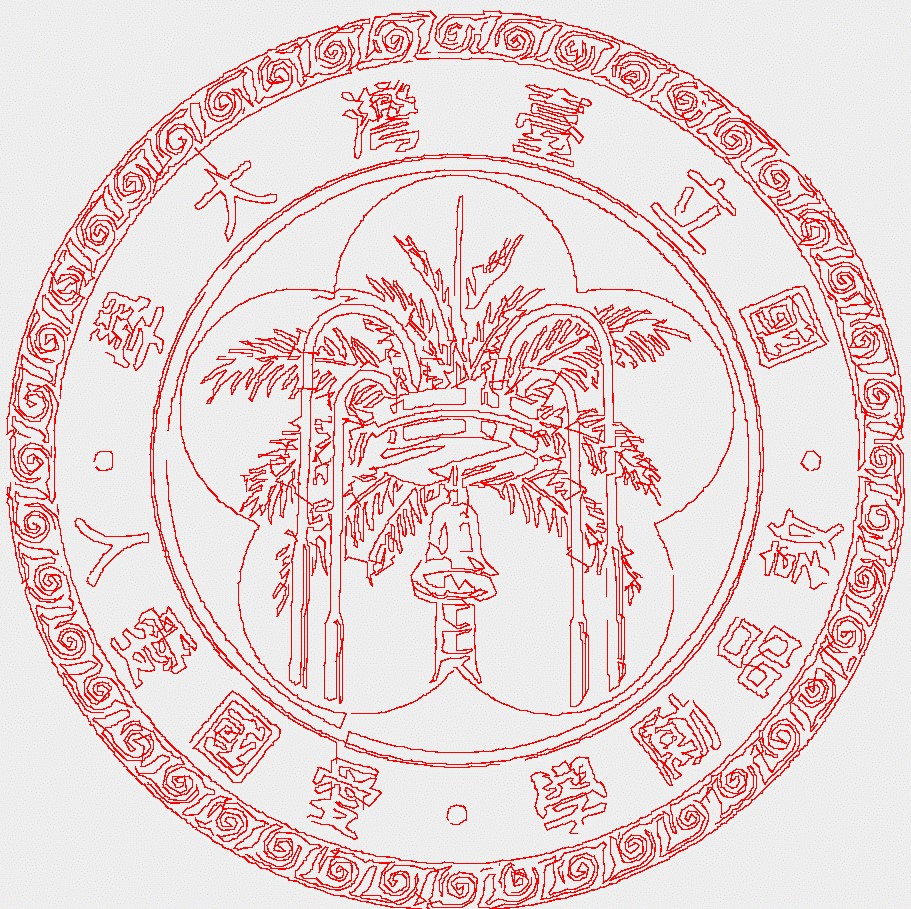
\includegraphics[width=120pt]{NTU r=0.4.jpg}
      \caption*{\textbf{圖\,8}\(\quad\)\(r=0.4\)\,時的輸出}
    \end{minipage}
    \quad
    \begin{minipage}{0.3\linewidth}
      \centering
      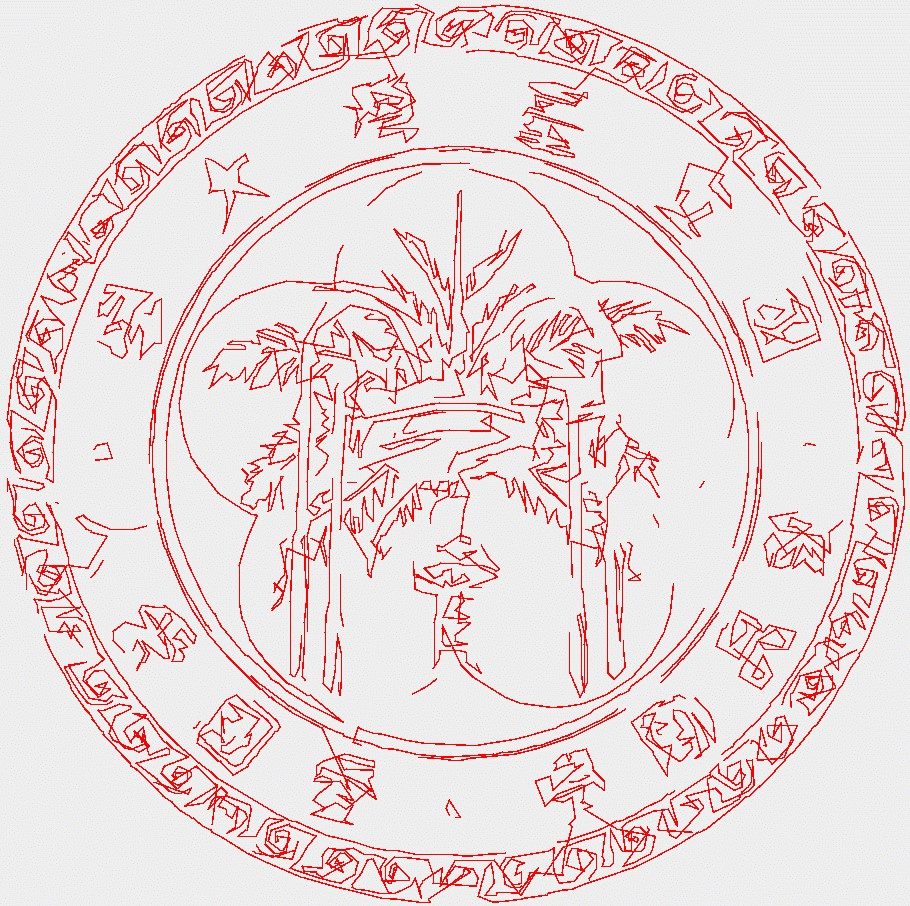
\includegraphics[width=120pt]{NTU r=0.1.jpg}
      \caption*{\textbf{圖\,9}\(\quad\)\(r=0.1\)\,時的輸出}
    \end{minipage}
  \end{figure}
  \noindent \\
  可以看到當\,\(r=0.7\)\,時,無論是文字抑或是紋路均與\,\(r=1\)\,時相差無幾;而當\,\(r=0.4\)\,時,圖片的重現效果也仍然意外地出色:即使僅使用了不到一半的像素點,整體的圖樣仍相當清晰,且所有的文字仍能被清楚辨認;最後於\,\(r=0.1\)\,的情況下,樣本數的嚴重不足使得圖片失真的情況過於嚴重,已經無法藉由提高\,\texttt{dist}\,之值修補圖片。
  \\\\
  因此我們可以證實在一定的壓縮程度下,圖片可以省去超過一半的容量且不失真。
  